% Preamble

\documentclass[12pt]{article}
\usepackage[pdftex]{graphicx}
\usepackage{geometry}
\usepackage[USenglish]{babel}
\usepackage[utf8]{inputenc}
\usepackage{fancyhdr}
\usepackage{float}
\usepackage{afterpage}
\usepackage{caption}
\usepackage{subcaption}
\usepackage{wrapfig}
\usepackage{booktabs}
\usepackage{lineno}
\usepackage{amssymb}
\usepackage{siunitx}

% Document parameters

\geometry{letterpaper, margin=1in}
\pagestyle{fancy}
\rhead{DISSERTATION PROPOSAL}
\lhead{Christopher M. Tasich}
\cfoot{\thepage}
\linespread{1}
\DeclareSIUnit\year{yr}
\DeclareSIUnit\foot{ft}
\setlength{\headheight}{15pt}

% Document
\begin{document}

\begin{titlepage}
	\begin{center}
		\vspace*{\fill}
		\textbf{{\LARGE Sediment model manuscript}}\\
		\line(1,0){300}\\
		Christopher M. Tasich\\
		Jonathan M. Gilligan\\
		Steven L. Goodbred\\
	\end{center}
	\vspace*{\fill}
\end{titlepage}

\section{Introduction}

\subsection{Overview}

Humans have always exploited nature for resources and, until recently, very little consideration has been given to the repercussions of these actions. Often human and natural systems are studied separately without a focus on the feedbacks between the two. However, as we move toward a global population of 10 billion people by 2050 \cite{unitednationsWorldPopulationProspects2017}, these links between these systems become increasingly important. Populations can no longer extract resources or alter the land without considering the repercussions of such actions. Furthermore, climate change and the associated sea level rise (SLR) will be significant stressors to coupled human and natural system.

In particular, low-lying deltas, such as the Ganges-Brahmaputra-Meghna (GBM) delta, face significant challenges as the human and natural systems are often tightly coupled. Here, small perturbations to one system can manifest as large perturbations to the other \cite{hoegh-guldbergImpacts5CGlobal2018}. Furthermore, Bengal has experienced extreme population growth and staggering land-use change due to development \cite{unitednationsWorldPopulationProspects2017}. As such, the GBM delta and the Bengal geopolitical region provide an incredible opportunity to study these types of interactions. In the context of this study, we will focus on the human alteration of landscapes in GBM delta and the coupled feedback response between the human and natural systems.

\subsection{Study Region}

The GBM delta has been populated for over 20,000 years and there is clear evidence of human alteration of the land beginning over 2,000 years ago. More recently, the region has experienced a significant population boom and it is now one the most densely populated regions on earth \cite{bangladeshbureauofstatistics2011PopulationHousing2011}. Often termed the "Green Delta," the region is one of the most fertile deltas in the world. Within the country of Bangladesh, \SI{>35}{\percent} of the population has built their livelihood around agriculture. This number grows to \SI{>45}{\percent} in rural areas \cite{bangladeshbureauofstatisticsReportHouseholdIncome2010}. As a result of this focus on agricultural in the GBM delta, large swaths of land have been converted to agricultural fields. This has significantly altered the massive flux of water and sediment flowing through the delta and into the Bay of Bengal. Furthermore, portions of southwest Bangladesh, rely on the sediment flux from the GBM mouth to maintain the landscape. We focus much of our research on Polder 32 in the tidally-dominated southwest of Bangladesh (Fig. \ref{fig:map}). Here, the human and natural systems are intimantely intertwined allowing us to easily observe and study the feedbacks between these systems. 

\begin{figure}[H]
	\center{\includegraphics[width=0.65\textwidth]
		{../figures/map.png}}
	\caption[Map of the Bengal Basin]{\label{fig:map} Map of the Bengal Basin. The white box indicates the location of Polder 32. A high resolution image of Polder 32 is in the right inset.}
\end{figure}

\subsection{Research Questions}

Here, we propose three broad categories of research related to the coupled human and natural systems found in the GBM delta. Within each section, we consider specific tractable questions to help answer the broader questions below.

\begin{enumerate}
	\item How do the tides and suspended sediment interact in southwest Bangladesh?
	\item How do changes in sediment aggradation patterns affect human decision-making and vice-versa?
	\item How do arsenic concentrations in the groundwater correlate spatially with stratigraphy?
\end{enumerate}

\section{A model of sediment accumulation}

\subsection{Motivation and Background}

The GBM river systems convey nearly \SI{1.1}{\giga\tonne\per\year} of sediment to the Bay of Bengal \cite{millimanGeomorphicTectonicControl1992}. Much of this sediment is deposited offshore in the subaerial delta, but nearly \SI{200}{\mega\tonne\per\year} is advected back onshore by strong semidiurnal tides. This tidally-dominated region is otherwise disconnected from the the fluvial system and relies solely on the tidal reworking of the sediment to maintain the landscape. Historically, mangroves swamps thrived here as the area is naturally inundated during spring high tides. The swamps were relatively uninhabited by humans, though other wildlife abounded. In the 1960s, some of these landscapes were converted to polders, or embanked islands, for agricultural expansion. While initially providing a boon to the region, the embankments have had the unintended consequence of starving the polder interiors of new sediment brought by the tides. As a result, the polder interiors have subsided due to compaction and tectonic subsidence and now some polder interiors sit as much as \SIrange{1.0}{1.5}{\meter} below mean high water \cite{auerbachFloodRiskNatural2015}. This offset contributes substantially to relative mean sea level (RMSL) rise, which threatens the livelihoods of the 40 million people living on these embanked landscapes. Below, we outline the current state of the polders and highlight two future scenarios that may impact the surface water and sediment dynamics of the region.

\subsubsection*{Depressed polders}

The most acute problem facing the polders is waterlogging during and following the monsoon season \cite{khadimIntegratedWaterResources2013a}. As most of the landscape is below the water level of the tidal channel, rainwater does not properly drain, leaving standing water and persistently wet soils within the polders. This lowers crop yields and consequently economic benefit to the polder inhabitants.

A rarer, but more devastating problem facing the polders, is the failure of the exterior embankments that prevent against tidal inundation. In 2009, Cyclone Aila devastated Polder 32 in Southwest Bangladesh when the embankments were breached in five locations. This resulted in the landscape being inundated to a mean depth of \SI{\sim 1}{\meter} for \SI{\sim 10}{\hour\per\day} for nearly two years \cite{auerbachFloodRiskNatural2015}. During this time, the inhabitants of Polder 32 lived in makeshift homes built along the already weakened embankments.

Tidal river management (TRM) is a possible solution to remediate the depressed polder landscapes. Using TRM, locals can allow for controlled inundation of the polder, which will replenish the land with nutrient-rich sediment. This inundation will prevent cultivation of crops for a period of time, though, presumably the land will slowly aggrade becoming more resilient with time. In the low-lying Beels region, north of Khulna, TRM has been implemented with varying success \cite{khadimIntegratedWaterResources2013a, shampaTidalRiverManagement2012, vanstaverenBringingTidesClosing2017}. However, there has been very little quantitative research into the natural mechanisms leveraged in TRM. Shampa and Pramanik \cite{shampaTidalRiverManagement2012} focused on tidal prism over which sediment may be dispersed. They found that TRM at Beel Jalalpur would be most successful with two link canals in order to maximize the tidal prism. Talchabhadel et al. \cite{talchabhadelExperimentalStudyTidal2017} constructed a two-dimensional unsteady flow model that focused on determining the most efficient breach size to maximize flow velocities and suspended sediment load. Neither focus on the feedback between tidal inundation and sediment accumulation as proposed in our study.

\subsubsection*{Changes in sediment supply}

Bangladesh and India have a strained history surrounding access to the Ganges and Brahmaputra Rivers. India has long sought to divert portions of these rivers for internal usage. The Farakka Barrage Project began diverting water from the Ganges in 1972. While the barrage only diverts \SI{<10}{\percent} of the total water of the Ganges, it has been criticized as raising salinity levels and causing siltation downstream \cite{gainImpactFarakkaDam2014}. More recently, India has proposed a large scale engineering project known as the Indian Rivers Inter-link, to link their river systems together via a network of canals and reservoirs. This may also serve to divert more water from Bangladesh. These conversations often focus on the impact on water flow across the border, but arguably of equal importance is the change in sediment flux. Higgins et al. \cite{higginsRiverLinkingIndia2018}  suggested a reduction in suspended sediment discharge of \SIrange{39}{75}{\percent} in the Ganges and \SIrange{9}{25}{\percent} in the Brahmaputra. The reduction in sediment could have devastating effects downstream, especially, in the tidal regions of the delta that rely on sediment aggradation to maintain pace with mean high water levels.

\subsubsection*{Changes in sea level}

Southwest Bangladesh has experienced RMSL rise of \SIrange{2.8}{8.8}{\milli\meter\per\year} as measured from three tide gauges between Khulna and Hiron Point \cite{pethickRapidRiseEffective2013}. Previous studies have suggested that modest rates of eustatic SLR may lead to large scale inundation as far north as Dhaka \cite{huqSeaLevelRiseBangladesh1995,aliVulnerabilityBangladeshClimate1996,sarwarImpactsSeaLevel2005}. However, these studies view the land surface elevation as static and do not consider the feedback of sediment aggradation due to tidal inundation. Presently, as a result of an abundant sediment supply, the repeated tidal inundation allows the landscape to maintain pace with RMSL rise. Despite the current resilience of the system, as RMSL rates increase, there may be a tipping point at which the landscape can no longer maintain pace.

\subsubsection*{Simulating changes to the tidal system}

Here, we propose a simple zero-dimensional, numerical model of tidal inundation and the resulting sediment aggradation at a point on the tidal platform. We attempt to answer three questions using this model.

\begin{enumerate}
	\item Under present conditions, how much time is needed to re-equilibrate the depressed polder elevations to the natural elevation (i.e. mean high water)?
	\item How does varying suspended sediment supply change the accumulation rate?
	\item At what rate of RMSL rise, does the tidal platform become permanently inundated?
\end{enumerate}

\subsection{Methods}

\subsubsection*{Numerical model}

We modeled tidal platform elevation ($\zeta$) using a zero-dimensional mass balance model using the basic formulation provided by Krone \cite{kroneMethodSimulatingMarsh1987} and further refined by Allen \cite{allenSaltmarshGrowthStratification1990}, French \cite{frenchNumericalSimulationVertical1993}, and Temmerman et al. \cite{temmermanModellingLongtermTidal2003,temmermanModellingEstuarineVariations2004}. The rate of tidal platform elevation is described as
\begin{equation}\label{eq1}
	\frac{d \zeta}{d t} = \frac{d S_M}{d t} + \frac{d S_O}{d t} + \frac{d P}{d t} + \frac{d M}{d t},
\end{equation}
where $S_M$ is mineral sedimentation, $S_O$ is organic matter sedimentation, $P$ is compaction, and $M$ is tectonic subsidence. Each term of equation \ref{eq1} can be further expanded.

We approximate $S_M$ as
\begin{equation}\label{eq2}
	S_M(t) = \int{\frac{w_{s}C(t)}{\rho}dt},
\end{equation}
where $w_s$ is the characteristic settling velocity of a grain given by Stokes' law, $C$ is the depth-averaged suspended sediment concentration in the water column, and $\rho$ is the dry bulk density of the sediment. We assume there is no resuspension of mineral sediment which is consistent with Krone's \cite{kroneMethodSimulatingMarsh1987} initial approximation.

We capture the temporal variation of $C$ during one tidal cycle through the mass balance given as
\begin{equation}\label{eq3}
	\frac{d[h(t)-\zeta]C(t)}{dt} = -w_sC(t)+C_{in}\frac{dh}{dt},
\end{equation}
where $h$ is the height of the water column and $C_{in}$ is the incoming suspended sediment concentration of the adjacent water column.

We are more uncertain of $C_{in}$. Most studies \cite{kroneMethodSimulatingMarsh1987,allenSaltmarshGrowthStratification1990,frenchNumericalSimulationVertical1993,frenchTidalMarshSedimentation2006} used a constant $C_{in}$ while Temmerman et al. \cite{temmermanModellingLongtermTidal2003,temmermanModellingEstuarineVariations2004} considered $C_{in}$ as a positive linear function of inundation height above the platform. For our study, $C_{in}$ varies significantly within a tidal cycle, seasonally, and between spring and neap tides. Conceptually, $C_{in}$ can be given as
\begin{equation}\label{eq4}
	C_{in} = f(SSC, h),
\end{equation}
though the exact relationships are unclear. Using new field observations \cite{haleObservationsScalingTidal2019}, we will determine the best way to approximate $C_{in}$.

In previous model runs, we focused exclusively on $S_M$ as it dominates equation \ref{eq1}. $S_O$, $P$, and $M$ were all set to zero. We will evaluate the need to incorporate these terms and determine the appropriate functions to approximate each.

\subsubsection*{Model inputs}

Field observations informed our model inputs ($h$, $w_s$, $C_{in}$, and $\rho$). We observed tidal height, grain size, suspended sediment concentration (SSC), and dry bulk density around Polder 32 over multiple field seasons from 2011 to 2016 \cite{auerbachFloodRiskNatural2015,haleObservationsScalingTidal2019}.

For $h$, we extracted one year of contiguous tidal data from from a pressure sensor deployed within the tidal channel near Polder 32. We replicated this tidal curve for each subsequent year for the length of the model run. In order to simulate RMSL rise, the subsequent year tidal curves were increased at a linear rate. Future model runs will include a more sophisticated approach to simulating RMSL rise. Rahmstorf \cite{rahmstorfSemiEmpiricalApproachProjecting2007} highlighted a semi-empirical approach to eustatic SLR that may serve to better approximate the projected tidal curve for the region.

For $w_s$, we first determined a characteristic grain size for the region. The median grain size was measured in multiple locations around Polder 32 and within the natural mangrove forest. We then used Stoke's Law to determine $w_s$ for our model.

For $C_{in}$, we use observed values of SSC from Hale et al. \cite{haleObservationsScalingTidal2019} that are characteristic of the tidal channels in the region. Similar to Temmerman et al. \cite{temmermanModellingLongtermTidal2003,temmermanModellingEstuarineVariations2004}, we scaled the observed tidal channel SSC by a k-factor as the flood waters are expected to have a lower SSC than the tidal channel due to lower flow velocities. For our preliminary study, we use a k-factor of 0.7. In future model iterations, we will better explore this relationship and determine an appropriate k-factor.

For $\rho$, we used values derived from conversations with Steven Goodbred and Carol Wilson.

\subsubsection*{Monte Carlo analysis of tidal river management}

We conducted a Monte Carlo analysis to capture model sensitivity to parameters and to determine the confidence intervals for simulating TRM over \SI{50}{\year}. We ran many iterations ($n = 10,000$) of the model with a time step of three-hours. With each iteration, we selected values of grain size, $\rho$, and $SSC$ from normal distributions (Table \ref{fig:tbl1}). The selected grain size was then converted to a settling velocity ($w_s$) using Stokes' Law. With each draw, there was a small chance that a parameter value would be negative. In these cases, we redrew until the parameter value was positive. Different distributions may be more appropriate and avoid this issue.

\begin{table}[H]
	\centering
	\caption[Distribution parameters for sediment model inputs]{\label{fig:tbl1} Distribution parameters for sediment model inputs.}
	\begin{tabular}{cccc}
		\hline
		Parameter  & Unit                              & Mean      & Std. Dev. \\ \hline
		grain size & \SI{}{\milli\meter}               & \SI{0.03} & 0.01      \\
		$\rho$     & \SI{}{\kilo\gram\per\cubic\meter} & 700       & 100       \\
		SSC        & \SI{}{\gram\per\liter}            & 0.4       & 0.1       \\ \hline
	\end{tabular}
\end{table}


\subsubsection*{Future simulations}

Using the same methodology described above, we will simulate changes in elevation to both the poldered and natural systems due to (1) RMSL rise and (2) changes in the sediment flux due to the Indian Rivers Inter-link. In order to simulate RMSL rise, we will adjust the tidal curve ($h$) using both linear rates and the semi-empirical approach presented by Rahmstorf \cite{rahmstorfSemiEmpiricalApproachProjecting2007}. For the Indian Rivers Inter-link scenario, we will adjust the suspended sediment concentration ($SSC$) to simulate a decrease in sediment flux from India as outlined by Higgins et al. \cite{higginsRiverLinkingIndia2018}.

\subsection{Preliminary results}

The base condition numerical model shows that under current polder conditions, the median simulation of elevations returns to the natural elevation after \SI{\sim 7}{\year} (Fig. \ref{fig:monte_carlo}). Though, some of the model runs take a considerably more time to re-equilibrate.

\begin{figure}[H]
	\center{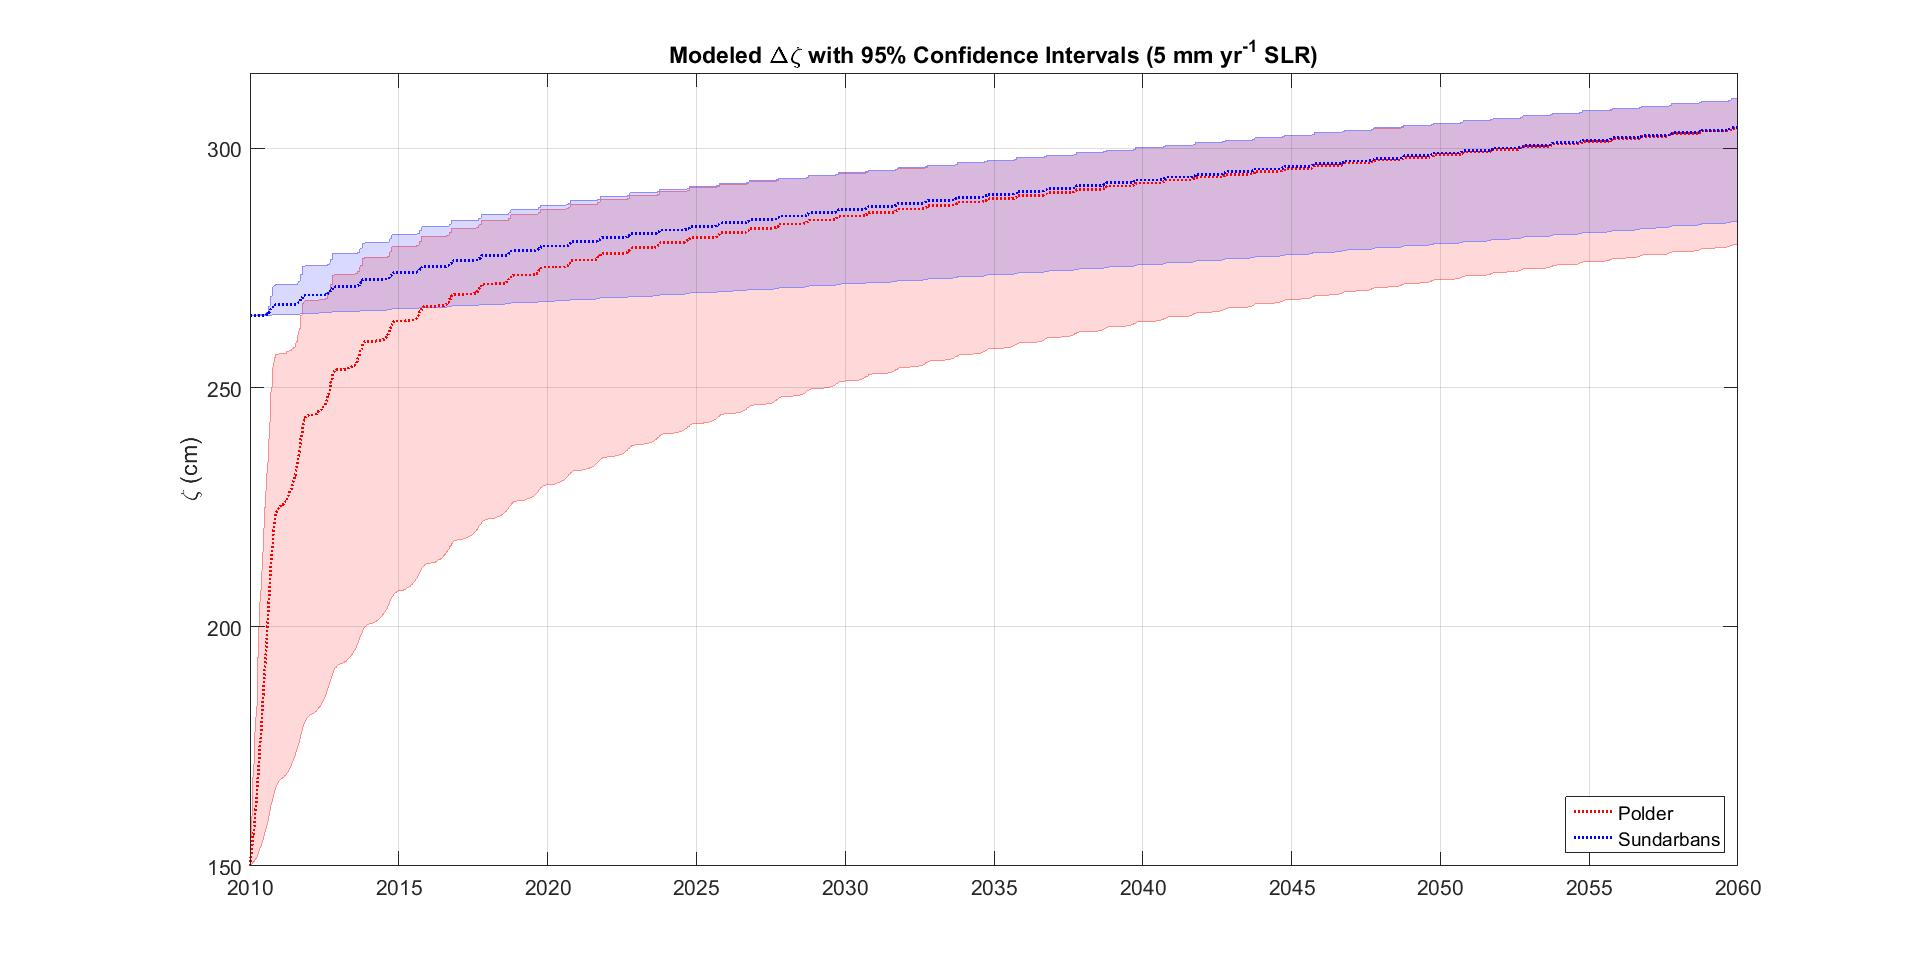
\includegraphics[width=\textwidth]
		{../figures/dZ.jpg}}
	\caption[Modeled platform elevations from 2010 to 2060]{\label{fig:monte_carlo} Modeled platform elevations from 2010 to 2060 for both the poldered and natural environments. Most of the model runs return to the natural level very quickly with some taking the nearly the entire \SI{50}{\year}.}
\end{figure}

We found that the model was highly sensitive to settling velocities (Fig. \ref{fig:mc_partial_corr}). Given this, we need to careful consider the grain size distribution used for the model. It may be necessary to include multiple grain sizes.

\begin{figure}[H]
	\begin{minipage}{0.49\linewidth}
		\centering
		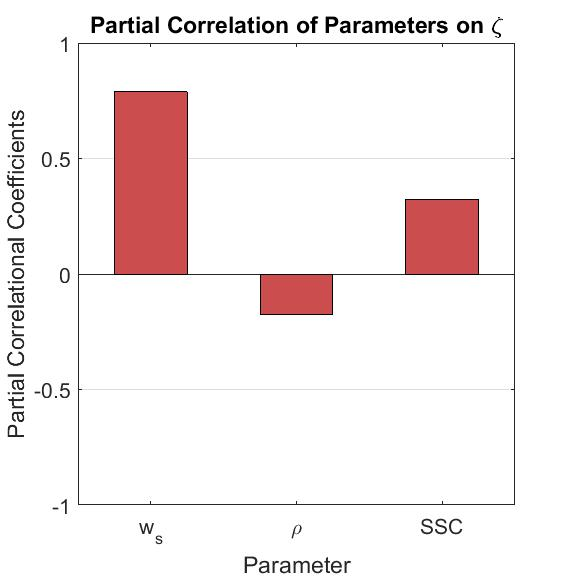
\includegraphics[width=\textwidth]{../figures/sens_mc.jpg}
	\end{minipage}
	\hfill
	\begin{minipage}{0.49\linewidth}
		\centering
		\setlength\tabcolsep{0pt}
		\setlength\tabcolsep{20px}
		\begin{tabular}{cc}
			\hline
			Parameter & Elevation \\ \hline
			$w_s$     & 0.79      \\
			$\rho$    & -0.17     \\
			$SSC$     & 0.32      \\ \hline
		\end{tabular}
	\end{minipage}
	\caption[Partial correlational coefficients of the sediment model]{\label{fig:mc_partial_corr} Partial correlational coefficients for baseline Monte Carlo analysis. Changes in $w_s$ result in the largest change in elevation, while both $\rho$ and $SSC$ have smaller effects.}
\end{figure}

\subsection{Anticipated results}

Presently, our model shows that the system effectively maintains pace with moderate rates of RMSL rise. Within our model, increasing RMSL largely has a positive effect on elevation. As RMSL rise rates increase, the system is inundated more often allowing for higher rates of sediment accumulation. However, we would expect at some point, $w_s$ would not be able to compensate for extreme rates of RMSL rise.

One reason that the system has maintained pace with current rates of RMSL rise is due to an abundance of suspended sediment. The significant changes in the sediment flux from the Ganges and Brahmaputra highlighted by Higgins et al. \cite{higginsRiverLinkingIndia2018} may dramatically decrease the amount of suspended sediment available in tidal system. This can be expected to lower the rate of sediment accumulation and ultimately make the system less resilient to even small amounts of RMSL rise and, more catastrophically, storm surge.

In reality, these scenarios may play out together in a complex manner. At lower rates of RMSL rise, the system may actually benefit from increased inundation times. However, with high rates of RMSL rise and decreased suspended sediment, the system, more than likely, will drown and the shoreline will regress inland.

\pagenumbering{gobble}
\addcontentsline{toc}{section}{References}
\bibliographystyle{pnas-new}
\bibliography{dissertation_proposal}

\end{document}